%% We use `subfiles' package
\documentclass[preamble.tex]{subfiles}
\begin{document}

\clearpage

\chapter{Array Fusion}
\label{ch:Fusion}

Suppose we have the following computation to perform:

\begin{hscode}
sum (zipWith (*) xs ys)
\end{hscode}

A person familiar with the fundamentals of functional programming is likely to spot the computation of the dot product of two vectors in this snippet of \Haskell code. Indeed, the @zipWith@ list combinator\icomb will element-wise multiply the two vectors @xs@ and @ys@. Quite expectedly the @sum@ combinator will sum the elements of the resulting vector into a scalar value yielding the dot product of @xs@ and @ys@.

This one-liner was an attempt to develop the motivation for the high-level view on numeric computations. It may seem reasonable to replace the lists with arrays and reimplement the same high-level interface in terms of traditional arrays to avoid random memory access penalties as in the case of lists.

Providing an instantly familiar interface without compromising performance has been one of the goals of the \name{Data Parallel Haskell (DPH)}\idph project \cite{PLKC08,CLP+07}. The work described in this essay has been carried out in the context of this project. It will be discussed in more detail in section \ref{sec:DPH}.

However, even if we replaced the lists with arrays and gave efficient implementations to @sum@ and @zipWith@, the resulting algorithm is still likely to be slower than one written by hand in a language such as \C. The @zipWith@ combinator \*produces* an \*intermediate array*\iintermediate containing the element-wise product of the two input vectors. It is immediately \*consumed* by @sum@, yielding the final (scalar) value. Thus the algorithm performs two traversals and allocates another array of the size of the input arrays.

To illustrate the benefit of Array Fusion let us turn to the implementation of same algorithm expressed in \C:


\begin{ccode}
double dotProduct (double xs[], double ys[], int len) {
	// zipWith
	double* temp = malloc(len * sizeof(double));
	for(int i = 0; i < len; i++)
		temp[i] = xs[i] * ys[i];

	// sum
	double result = 0;
	for(int i = 0; i < len; i++)
		result += temp[i];

	return result;
}
\end{ccode}


We immediately notice that both loops iterate over the same \*range* of indices and we could hence perform it as one loop. The two loops are said to have the same \*rate*\irate (the term used more recently in the context of loop fusion in \Haskell \cite{BenLippmeier:2014jc}).


\begin{ccode}
double* temp = malloc(len * sizeof(double));
double result = 0;
for(i = 0; i < len; i++) {
	temp[i] = xs[i] * ys[i];
	result += temp[i];
}
\end{ccode}


\begin{bluebox}
The process of finding and exploiting the opportunities for merging multiple loops into one is referred to as \term{loop fusion}.\ifusion
\end{bluebox}


However, this does not completely bypass the allocation of an intermediate array.\iintermediate Clearly, the intermediate array is redundant and the intermediate value @temp@ could just be a \*scalar* as in the following:


\begin{ccode}
double temp; // temp has become scalar
double result = 0;
for(int i = 0; i < len; i++) {
	temp = xs[i] * ys[i];
	result += temp;
}
\end{ccode}


\begin{bluebox}
The optimisation that removes the need for temporary arrays by replacing them with scalars is called \term{scalarisation}.\idx{scalarisation}
\end{bluebox}


It is a special case of \term{array contraction}.\idx{array contraction} Array contraction optimisation attempts to remove a \*dimension* from the array. In this particular case we contracted a one dimensional array to a scalar, hence \*scalarisation*. However, in the examples with arrays of higher dimensions the dimension could just be reduced, and not eliminated entirely. We will see examples of that in the upcoming chapters when we discuss \*segmented array combinators*.\isegcomb This concept is taken even further in multi-dimensional array systems such as \name{Repa} \cite{KCL+10} and \name{Accelerate} \cite{CKL+11}.


\begin{bluebox}
\term{Loop Fusion} and \term{Array Contraction} optimisation are collectively referred to as \term{Array Fusion}.
\end{bluebox}


Another term for this commonly encountered in literature is \term{deforestation},\idx{deforestation} first coined by Philip Wadler in \cite{Wad90}.


In the remainder of this chapter I outline the reasons which led me to the line of work described in this thesis.



%\clearpage
%\section{Types of collective array operations}
%\label{sec:combinator-types}

%In this section I present a classification of collective array operations\icollop that were of primary importance for this project. The classification is based on how the combinators consume\icomb their inputs and produce outputs.

%It is by no means the only way to classify the combinators. However, the analysis is aimed to showcase the different ways in which array combinators may interact with each other is a user program.

%While the discussion of the context of the work and the justification of the choice of combinators is left until the next chapter, we will attempt to put the currently available fusion systems in perspective and determine the combinators and programs for which they perform less effectively.


\clearpage
\section{The problem statement}
\label{sec:problems}

In this section I identify several types of fusion as well as the shortcomings of the previously available fusion systems which motivated the search for a fresh approach.

I will make many references to the \StreamFusion\isf (\cite{CLS07}, \cite{CSL06}, \cite{VectorStreamFusion}) framework in my discussion as one of the most comprehensive fusion frameworks that exist for \Haskell. However, I also will implicitly or explicitly make references to \name{foldr/build} \cite{GLP93}, \name{Functional Array Fusion} \cite{CK01} since they all fall into the category of \term{equational fusion frameworks}.\ieqf Such fusion systems rely on adjacent term rewriting\irw (for example through the use of rewrite rules\irwrules \cite{PTH01}) and subsequent compiler optimisations to produce efficient code.

\StreamFusion and \name{foldr/build} fusion are covered more thoroughly in Appendix~\ref{sec:Equational-Fusion-Systems}.



\subsection{Simple pipeline fusion}
\label{sec:straight-line}

The most basic form of optimisation that is attempted by most fusion systems is @map/map@ fusion where a pipeline of @map@ combinators is transformed into a single @map@:

\begin{hscode}[mathescape]
map g $\circ$ map f $\mapsto$ map (g $\circ$ f)
\end{hscode}

However, @map@ is not the only combinator that can be chained together in a pipeline. @scan@ and @filter@, like @map@, both \*consume* one array and \*produce* another.
% are both \term{array transducers}\idx{transducer}, in that they \*consume* one array and \*produce* another.

In the simplest case, at the beginning of such a combinator pipeline there is a physical, or \term{manifest}\imanifest array, materialised in memory. However, there may also be a \term{pure producer} or a \term{generator}\igencomb instead. As such @replicate@, @enumerate@ and several others, generate an array from scalars or functions according to some rule.

Just like a pipeline does not necessarily start with a physical array, it may be concluded with a computation such as @fold@ yielding one scalar value.

The combinators discussed so far can be combined into a pipeline of operations where an array output of one combinator is fed directly as input to the next. Additionally, each combinator in the pipeline is able to consume the elements one by one at the \*rate* they are produced by the preceding combinator.

%Assuming that a computation is expressed a pipeline of combinators uninterrupted by \*branching* or \*control flow* are generally handled well by many existing fusion frameworks.

Such simple pipelines are generally handled well by most fusion frameworks. In particular the expressions presented in Figure~\ref{fig:simple-piplines} are all fusible by \StreamFusion \cite{CLS07} (and Appendix~\ref{sec:stream-fusion}) and \name{Functional Array Fusion} \cite{CK01}.

\begin{figure}
\begin{hscode}
let ys = map (/100)     let s = fold (+) 0       let ws = filter odd
       $ filter (>0)          $ map (^2)                $ map (+1)
       $ xs                   $ scan (*) 1              $ enumFromTo 1 10
                              $ zs
\end{hscode}

\begin{subfigure}{.33\textwidth}%
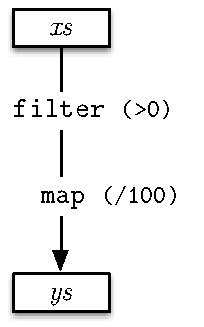
\includegraphics[center,scale=\omniscale]{img/DFD-simple-pipeline-a}%
\end{subfigure}%
\begin{subfigure}{.33\textwidth}%
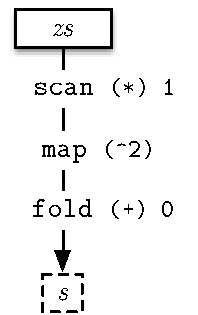
\includegraphics[center,scale=\omniscale]{img/DFD-simple-pipeline-b}%
\end{subfigure}%
\begin{subfigure}{.33\textwidth}%
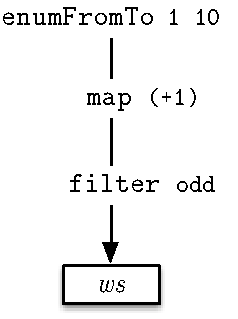
\includegraphics[center,scale=\omniscale]{img/DFD-simple-pipeline-c}%
\end{subfigure}%

\caption{Examples of simple combinator pipelines: \Haskell expressions (top) and their corresponding data flow graphs (bottom).}
\label{fig:simple-piplines}
\end{figure}


\subsection{Fusing into multiple consumers}
\label{sec:multiple-consumers}

In the previous section we have looked at \*uninterrupted* pipelines of combinators. Each intermediate array produced by a combinator was immediately consumed by \*exactly one* other combinator.

However, in some cases the output of a combinator may be consumed at two or more places in the program. Consider the example on Figure~\ref{fig:ratios}, showing a program computing, for each element, the ratio of the sum of all preceding elements to the current element. Because computing the ratio involves division operator, the input array is first filtered to exclude any zero elements.

The output of the @filter@ combinator is consumed by both the @scan@ to compute the partial sums and the @zipWith@ to give the final ratio. If one was to write this in \C, the resulting program could be expressed in a single loop.

Nevertheless, this program will not be fused by an equational fusion system.\ieqf Even though each pair of combinators could be fused individually (@zipWith@/@scan@, @zipWith@/@filter@, @scan@/@filter@) in this program the fusion will stop already after @filter@.

The reason for this is the following. If fused by \StreamFusion\isf (the approach for other fusion frameworks is similar), the program will be first expanded to the following\footnote{See Appendix~\ref{sec:stream-fusion} for the explanation of this expansion.}:

\begin{hscode}
let nz     = unstream $ filterS (/= 0) $ stream xs
    psums  = unstream $ scanS (+) 0    $ stream nz
    ratios = unstream $ zipWithS (/) (stream psums) (stream nz)
in  ratios
\end{hscode}

For fusion to take place the following rewrite rule\irwrules needs to apply:

$\langle \mathit{stream/unstream\ fusion}\rangle\, \forall stream\, (unstream\, s)\mapsto s$

Unfortunately, because @nz@ term is used in multiple places, \GHC will not inline its definition into its use sites. This is done to prevent work duplication. This crucial step will prevent the fusion from occurring.

\begin{figure}

\begin{subfigure}{.5\textwidth}%
\begin{hscode}
let nz     = filter (/= 0) xs
    psums  = scan (+) 0 nz
    ratios = zipWith (/) psums nz
in  ratios
\end{hscode}
\end{subfigure}%
%
\begin{subfigure}{.5\textwidth}%
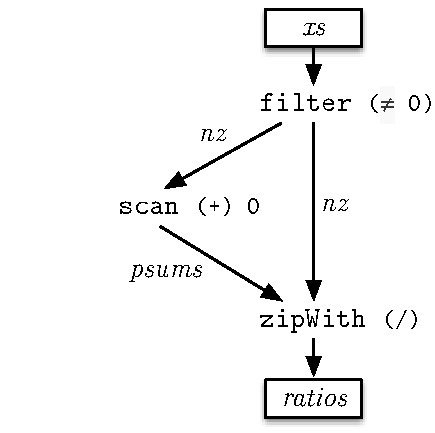
\includegraphics[center,scale=\omniscale]{img/DFD-ratios}%
\end{subfigure}%

\caption{\code{ratios} program illustrating the problem of multiple consumers (left) and the corresponding data flow graph (right).}
\label{fig:ratios}
\end{figure}


In the application of fusion to \DPH\idph we have discovered that this pattern of array consumption is recurring and if one of the principle factors contributing to reduced performance as far as fusion is concerned.

In particular the @filterMax@ program on Figure~\ref{fig:filterMax} is a simplified excerpt of the \DPH program computing convex hull of a set of points using \QuickHull\iqh algorithm. Given an array of @points@ it first computes the distance from each point to some line (not shown) by mapping @dist@ function. Then it finds all distances corresponding to points @above@ the line as well as the @farthest@ distance.

Again, in \C this whole computation could be expressed by one loop, traversing the @points@ array exactly once. However, @distances@ array is shared between @filter@ and @fold1@ consumers, preventing them from being fused by equational fusion frameworks into a single computation. In this example three array traversals would be performed instead of one, increasing memory traffic and memory footprint of the program.


\begin{figure}

\begin{subfigure}{.6\textwidth}%
\begin{hscode}
let dist (x,y) = ...
    distances  = map dist points
    above      = filter (> 0) distances
    farthest   = fold1 max distances
in  (above, farthest)
\end{hscode}
\end{subfigure}%
%
\begin{subfigure}{.4\textwidth}%
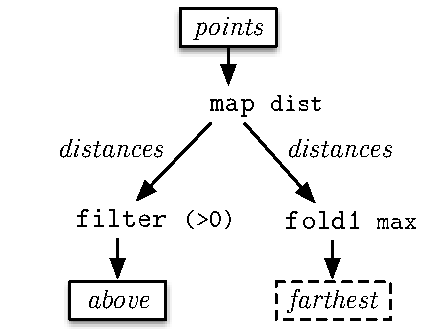
\includegraphics[center,scale=0.85]{img/filterMax-dataflow}%
\end{subfigure}%

\caption{\code{filterMax} program illustrating the problem of multiple consumers in DPH (left) and the corresponding data flow graph (right).}
\label{fig:filterMax}
\end{figure}


The inability to fuse branched data flow graphs where a single intermediate array is consumed by multiple combinators has proven to be critical to the application of fusion in \DPH and motivated the search for alternative approaches satisfying this requirement.

In the following section I discuss a problem with \StreamFusion which introduces runtime overhead in successfully fused programs.


\subsubsection{Duplicated counters}


In the beginning of this chapter the @zipWith@ combinator was used for point-wise multiplication of two vectors. Later it was used to compute point-wise ratios of two arrays (Figure~\ref{fig:ratios}).

While \StreamFusion is able to fuse \codemath{zipWith$N$} combinators where the input arrays are produced by \*independent*\footnote{As discussed in the previous section (\ref{sec:multiple-consumers}).} pipelines of combinators the generated code is not optimal.

For example, consider the following expression:

\begin{hscode}
zipWith3 (\ x y z -> (x + y) * z) xs ys zs
\end{hscode}

Assuming that @xs@, @ys@ and @zs@ are physical arrays in memory, \StreamFusion results in the following \name{GHC Core} code (adapted from \cite{FlowFusion}):

\begin{hscode}[numbers=left]
loop = \ i j k l s ->
  case >=# i len_xs of
    True  -> (# s, I# n #)
    False ->
      case indexIntArray# xs i of x ->
        case >=# j len_ys of
          True  -> (# s, I# n# #)
          False ->
            case indexIntArray# ys j of y ->
              case >=# k len_zs of
                True  -> (# s, I# n# #)
                False ->
                  case indexIntArray# zs k of z ->
                    loop (+# i 1) (+# j 1) (+# k 1) (+# l 1)
                      (writeIntArray# rs l (*# (+# x y) z) s)
\end{hscode}

Even though the arrays are consumed in lockstep, \StreamFusion introduces a separate counter for each input array (@i@, @j@ and @k@) as well as the output index variable @l@. \StreamFusion is unable to replace all four with one counter based on the fact that @i = j = k = l@. Not only this introduces extra bounds checks on lines 2, 6 and 10 and increments on line 14, but also increases register pressure. At present \GHC compiler is unable to identify the invariant @i = j = k = l@ and remove the redundant variables either.

In \DPH\idph it is not uncommon to to encounter point-wise processing of a much larger number of arrays. For example, the \QuickHull example mentioned in the previous section and discussed more thoroughly in Chapter~\ref{ch:results}, processes as many as 6 arrays using the @zipWith6@ combinator.

\name{Functional Array Fusion}\ifaf is able to fuse \codemath{zipWith$N$} combinators without introducing repeated counter variable but is overall a more fragile system than \StreamFusion as it relies on more complex rewrite to function. \name{foldr/build}\ishortcut fusion is unable to fuse point-wise operations altogether.

The problem of duplicated loop counters was an important problem solved by the proposed \LiveFusion system to avoid the overhead of performing extra arithmetic operations in the tight loop and reduce register pressure.

\todo{Related work, Discussion}

In following chapter I will introduce the reader to the \DPH project in order to see the applicability of array fusion to a particular.


\IfNotCompilingAll{\bibliography{bib}}


\end{document}